\section{Overview}

This tutorial provides the third protocol from our recent publication \citep{Hoehna2017a}.
The first protocol is described in the \href{https://github.com/revbayes/revbayes_tutorial/raw/master/tutorial_TeX/RB_CTMC_Tutorial/RB_CTMC_Tutorial.pdf}{Substitution model tutorial} and the second protocol is described in the \href{https://github.com/revbayes/revbayes_tutorial/raw/master/tutorial_TeX/RB_Partition_Tutorial/RB_Partition_Tutorial.pdf}{Partitioned data analysis tutorial}.

This tutorial demonstrates some general principles of Bayesian model comparison, which is based on estimating the marginal likelihood of competing models and then comparing their relative fit to the data using Bayes factors.
We consider the specific case of calculating Bayes factors to select among different substitution models.

\subsection{Requirements}
We assume that you have read and hopefully completed the following tutorials:
\begin{itemize}
\item \href{https://github.com/revbayes/revbayes_tutorial/raw/master/tutorial_TeX/RB_Getting_Started/RB_Getting_Started.pdf}{Getting started}
\item \href{https://github.com/revbayes/revbayes_tutorial/raw/master/tutorial_TeX/RB_Intro_Tutorial/RB_Intro_Tutorial.pdf}{\Rev basics}
\item \href{https://github.com/revbayes/revbayes_tutorial/raw/master/tutorial_TeX/RB_Rev_Tutorial/RB_Rev_Tutorial.pdf}{\Rev syntax}
\item \href{https://github.com/revbayes/revbayes_tutorial/raw/master/tutorial_TeX/RB_CTMC_Tutorial/RB_CTMC_Tutorial.pdf}{Substitution models}
\end{itemize}
Note that the \href{https://github.com/revbayes/revbayes_tutorial/raw/master/tutorial_TeX/RB_Intro_Tutorial/RB_Intro_Tutorial.pdf}{\Rev basics tutorial} introduces the basic syntax of \Rev but does not cover any phylogenetic models.
We tried to keep this tutorial very basic and introduce all the language concepts and theory on the way.
You may only need the \href{https://github.com/revbayes/revbayes_tutorial/raw/master/tutorial_TeX/RB_Rev_Tutorial/RB_Rev_Tutorial.pdf}{\Rev syntax tutorial} for a more in-depth discussion of concepts in \Rev.



%%%%%%%%
%%   Data   %%
%%%%%%%%
\section{Data and files}

We provide the data file that we will use in this tutorial.
Of course, you may want to use your own dataset instead.
In the \cl{data} folder, you will find the following file:
\begin{itemize}
\item
\cl{primates\_and\_galeopterus\_cytb.nex}: Alignment of the \textit{cytochrome b} subunit from 23 primates representing 14 of the 16 families (\textit{Indriidae} and \textit{Callitrichidae} are missing).
\end{itemize}



\section{Introduction}

For most sequence alignments, several (possibly many) substitution models of varying complexity are plausible \emph{a priori}.
We therefore need a way to objectively identify the model that balances estimation bias and inflated error variance associated with under- and over-parameterized models, respectively.
Increasingly, model selection is based on \emph{Bayes factors} \citep[\EG][]{Suchard2001,Lartillot2006,Xie2011,Baele2012,Baele2013}, which involves first calculating the marginal likelihood of each candidate model and then comparing the ratio of the marginal likelihoods for the set of candidate models.

 
Given two models, $M_0$ and $M_1$, the Bayes-factor comparison assessing the relative fit of each model to the data, $BF(M_0,M_1)$, is:
$$BF(M_0,M_1) = \frac{\mbox{posterior odds}}{\mbox{prior odds}}.$$
The posterior odds is the posterior probability of $M_0$ given the data, $\mathbf X$, divided by the posterior odds of $M_1$ given the data:
$$\mbox{posterior odds} = \frac{\mathbb{P}(M_0 \mid \mathbf X)}{\mathbb{P}(M_1 \mid \mathbf X)},$$
and the prior odds is the prior probability of $M_0$ divided by the prior probability of $M_1$:
$$\mbox{prior odds} = \frac{\mathbb{P}(M_0)}{\mathbb{P}(M_1)}.$$
Thus, the Bayes factor measures the degree to which the data alter our belief regarding the support for $M_0$ relative to $M_1$ \citep{Lavine1999}:
\begin{align}\label{BFeq1}
BF(M_0,M_1) = \frac{\mathbb{P}(M_0 \mid \mathbf X, \theta_0)}{\mathbb{P}(M_1 \mid \mathbf X, \theta_1)} \div \frac{\mathbb{P}(M_0)}{\mathbb{P}(M_1)}. 
\end{align}
Note that interpreting Bayes factors involves some subjectivity.
That is, it is up to \textsl{you} to decide the degree of your belief in $M_0$ relative to $M_1$. 
Despite the absence of an absolutely objective model-selection threshold, we can refer to the scale \citep[outlined by][]{Jeffreys1961} that provides a ``rule-of-thumb'' for interpreting these measures (Table \ref{bftable}).
\begin{table}[h]
\centering
\caption{\small The scale for interpreting Bayes factors by Harold \citet{Jeffreys1961}.} 
\label{bftable}
\begin{tabular}{l c c c}
\hline
\multicolumn{1}{r}{{Strength of evidence}} & \multicolumn{1}{l}{\textbf{$BF(M_0, M_1)$}} & \multicolumn{1}{l}{\textbf{log($BF(M_0, M_1)$)}} &  \multicolumn{1}{l}{\textbf{$\text{log}_{10}$($BF(M_0, M_1)$)}}\\ 
\hline
Negative (supports $M_1$) & $<1$ & $<0$ & $<0$\\
Barely worth mentioning & $1$ to $3.2$ & $0$ to $1.16$ & $0$ to $0.5$\\
Substantial & $3.2$ to $10$ & $1.16$ to $2.3$ & $0.5$ to $1$ \\
Strong & $10$ to $100$ & $2.3$ to $4.6$ & $1$ to $2$ \\
Decisive& $>100$ & $>4.6$ & $>2$ \\
\hline
\multicolumn{3}{l}{{\scriptsize{For a detailed description of Bayes factors see \citet{Kass1995}}}} 
\end{tabular}
\end{table}


Unfortunately, it is generally not possible to directly calculate the posterior odds to prior odds ratios.
However, we can further define the posterior odds ratio as:
\begin{align*}
\frac{\mathbb{P}(M_0 \mid \mathbf X)}{\mathbb{P}(M_1 \mid \mathbf X)} = \frac{\mathbb{P}(M_0)}{\mathbb{P}(M_1)} \frac{\mathbb{P}(\mathbf X \mid M_0)}{\mathbb{P}(\mathbf X \mid M_1)},
\end{align*}
where $\mathbb{P}(\mathbf X \mid M_i)$ is the \textit{marginal likelihood} of the data (this may be familiar to you as the denominator of Bayes Theorem, which is variously referred to as the \textit{model evidence} or \textit{integrated likelihood}).
Formally, the marginal likelihood is the probability of the observed data ($\mathbf X$) under a given model ($M_i$) that is averaged over all possible values of the parameters of the model ($\theta_i$) with respect to the prior density on $\theta_i$
\begin{align}\label{margeLike}
\mathbb{P}(\mathbf X \mid M_i) = \int \mathbb{P}(\mathbf X \mid \theta_i) \mathbb{P}(\theta_i)dt.
\end{align}
This makes it clear that more complex (parameter-rich) models are penalized by virtue of the associated prior: each additional parameter entails integration of the likelihood over the corresponding prior density.  
If you refer back to equation \ref{BFeq1}, you can see that, with very little algebra, the ratio of marginal likelihoods is equal to the Bayes factor:
\begin{align}\label{bfFormula}
BF(M_0,M_1) = \frac{\mathbb{P}(\mathbf X \mid M_0)}{\mathbb{P}(\mathbf X \mid M_1)} = \frac{\mathbb{P}(M_0 \mid \mathbf X, \theta_0)}{\mathbb{P}(M_1 \mid \mathbf X, \theta_1)} \div \frac{\mathbb{P}(M_0)}{\mathbb{P}(M_1)}. 
\end{align}
Therefore, we can perform a Bayes factor comparison of two models by calculating the marginal likelihood for each one. % Simple as pie, right?
Alas, exact solutions for calculating marginal likelihoods are not known for phylogenetic models (see equation \ref{margeLike}), thus we must resort to numerical integration methods to estimate or approximate these values. 
In this exercise, we will estimate the marginal likelihood for each partition scheme
using both the stepping-stone \citep{Xie2011,Fan2011} and path sampling estimators \citep{Lartillot2006, Baele2012}. 



\bigskip
\subsection{Substitution Models} 

The models we use here are equivalent to the models described in the previous exercise on substitution models (continuous time Markov models).
To specify the model please consult the previous exercise. Specifically, you will need to specify the following substitution models:
\begin{itemize}
\item Jukes-Cantor (JC) substitution model \citep{Jukes1969}
\item Hasegawa-Kishino-Yano (HKY) substitution model \citep{Hasegawa1985}
\item General-Time-Reversible (GTR) substitution model \citep{Tavare1986}
\item Gamma (+G) model for among-site rate variation \citep{Yang1994a}
\item Invariable-sites (+I) model \citep{Hasegawa1985}
\end{itemize}


\bigskip
\subsection{Estimating the Marginal Likelihood}

We will estimate the marginal likelihood of a given model using a `stepping-stone' (or `path-sampling') algorithm.
These algorithms are similar to the familiar MCMC algorithms, which are intended to sample from (and estimate) the joint posterior probability of the model parameters.
Stepping-stone algorithms are like a series of MCMC simulations that iteratively sample from a specified number of distributions that are discrete steps between the posterior and the prior probability distributions.
The basic idea is to estimate the probability of the data for all points between the posterior and the prior---effectively summing the probability of the data over the prior probability of the parameters to estimate the marginal likelihood. 
Technically, the steps correspond to a series of \cl{powerPosteriors()}, where the likelihood is iteratively raised to a series of numbers between 1 and 0 (Figure~\ref{fig:ss}).
When the likelihood is raised to the power of 1 (typically the first stepping stone), samples are drawn from the (untransformed) posterior.
By contrast, when the likelihood is raised to the power of 0 (typically the last stepping stone), samples are drawn from the prior.
To perform a stepping-stone simulation, we need to specify (1) the number of stepping stones (power posteriors) that we will use to traverse the path between the posterior and the prior (\EG we specify 50 or 100 stones), (2) the spacing of the stones between the posterior and prior (\EG we may specify that the stones are distributed according to a beta distribution), (3) the number of samples (and their thinning) to be drawn from each stepping stone, and (4) the direction we will take (\IE from the posterior to the prior or vice versa).



\begin{figure}[h!]
\centering
\fbox{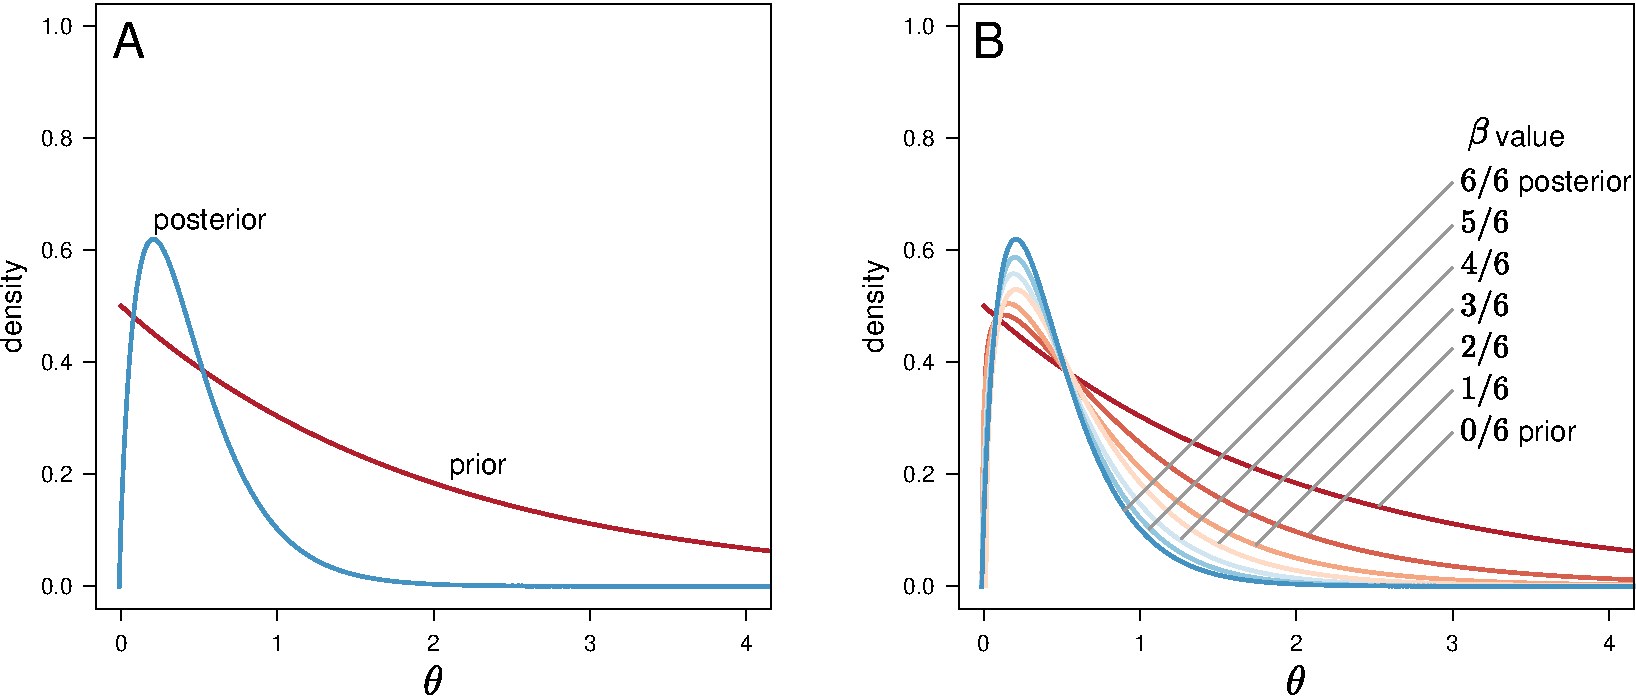
\includegraphics[width=\textwidth,angle=0]{\ResourcePath figures/ss.pdf}}
\caption{\small Estimating marginal likelihoods using stepping-stone simulation. 
Estimating the marginal likelihood involves integrating the likelihood of the data over the entire prior probability density for the model parameters.
MCMC algorithms target the posterior probability density, which is typically concentrated in a small region of the prior probability density (A).
Accordingly, standard MCMC simulation cannot provide unbiased estimates of the marginal likelihood because it will typically fail to explore most of the prior density.
(B) Stepping-stone algorithms estimate the marginal likelihood by means of a series of MCMC-like simulations, where the likelihood is iteratively raised to a series of powers, effectively forcing the simulation to more fully explore the prior density of the model parameters.
Here, six uniformly spaced stones span the posterior, where the power posterior is $\beta=6/6=1$, to the prior, where the power posterior is $\beta=0/6=0$.}
\label{fig:ss}
\end{figure}


This method computes a vector of powers from a beta distribution, then executes an MCMC run for each power step while raising the likelihood to that power. In this implementation, the vector of powers starts with 1, sampling the likelihood close to the posterior and incrementally sampling closer and closer to the prior as the power decreases. 

Just to be safe, it is better to clear the workspace (if you did not just restart \RevBayes):
{\tt \begin{snugshade*}
\begin{lstlisting}
clear()
\end{lstlisting}
\end{snugshade*}}

Now set up the model as in the previous exercise. You should start with the simple Jukes-Cantor substitution model. 
Setting up the model requires:
\begin{enumerate}
\item Loading the data and retrieving useful variables about it (\EG number of sequences and taxon names).
\item Specifying the instantaneous-rate matrix of the substitution model.
\item Specifying the tree model including branch-length variables.
\item Creating a random variable for the sequences that evolved under the \cl{PhyloCTMC}.
\item Clamping the data.
\item Creating a model object.
\item Specifying the moves for parameter updates.
\end{enumerate}

The following procedure for estimating marginal likelihoods is valid for any model in \RevBayes.
You will need to repeat this later for other models.
First, we create the variable containing the power-posterior analysis. 
This requires that we provide a model and vector of moves, as well as an output file name. 
The \cl{cats} argument sets the number of stepping stones.
{\tt \begin{snugshade*}
\begin{lstlisting}
pow_p = powerPosterior(mymodel, moves, monitors, "output/model1.out", cats=50) 
\end{lstlisting}
\end{snugshade*}}

We can start the power-posterior analysis by first burning in the chain and and discarding the first 10000 states.  
This will help ensure that analysis starts from a region of high posterior probability, rather than from some random point.
{\tt \begin{snugshade*}
\begin{lstlisting}
pow_p.burnin(generations=10000,tuningInterval=1000)
\end{lstlisting}
\end{snugshade*}}

Now execute the run with the \cl{.run()} function:
{\tt \begin{snugshade*}
\begin{lstlisting}
pow_p.run(generations=1000)  
\end{lstlisting}
\end{snugshade*}}

Once the power posteriors have been saved to file, create a stepping stone sampler. 
This function can read any file of power posteriors and compute the marginal likelihood using stepping-stone sampling. 
{\tt \small \begin{snugshade*}
\begin{lstlisting}
ss = steppingStoneSampler(file="output/model1.out", powerColumnName="power", likelihoodColumnName="likelihood")
\end{lstlisting}
\end{snugshade*}}

These commands will execute a stepping-stone simulation with 50 stepping stones, sampling 1000 states from each step. 
Compute the marginal likelihood under stepping-stone sampling using the member function \cl{marginal()} of the \cl{ss} variable and record the value in Table \ref{tab:ml_cytb}.
{\tt \begin{snugshade*}
\begin{lstlisting}
ss.marginal() 
\end{lstlisting}
\end{snugshade*}}

Path sampling is an alternative to stepping-stone sampling and also takes the same power posteriors as input. 
{\tt \small \begin{snugshade*}
\begin{lstlisting}
ps = pathSampler(file="output/model1.out", powerColumnName="power", likelihoodColumnName="likelihood")
\end{lstlisting}
\end{snugshade*}}

Compute the marginal likelihood under stepping-stone sampling using the member function \cl{marginal()} of the \cl{ps} variable and record the value in Table \ref{tab:ml_cytb}.
{\tt \begin{snugshade*}
\begin{lstlisting}
ps.marginal() 
\end{lstlisting}
\end{snugshade*}}

\noindent \\ \impmark As an example we provide the file \textbf{RevBayes\_scripts/marginalLikelihood\_JukesCantor.Rev}.

\begin{framed}
We have kept this description of how to use stepping-stone-sampling and path-sampling very generic and did not provide the information about the model here.
Our main motivation is to show that the marginal likelihood estimation algorithms are independent of the model.
Thus, you can apply these algorithms to any	model, \EG relaxed clock models and birth-death models, as well.
\end{framed}



\subsection{Exercises}

\begin{itemize}
\item Compute the marginal likelihoods of the \textit{cytb} alignment for the following substitution models:
\begin{itemize}
\item Jukes-Cantor (JC) substitution model
\item Hasegawa-Kishino-Yano (HKY) substitution model
\item General-Time-Reversible (GTR) substitution model
\item GTR with gamma distributed-rate model (GTR+G)
\item GTR with invariable-sites model  (GTR+I)
\item GTR+I+G model
\end{itemize}
\item Enter the marginal likelihood estimate for each model in the corresponding cell of Table~\ref{tab:ml_cytb}.
%\item Repeat the above marginal likelihood analyses for the \textit{mt-COX2 gene} and enter results in Table~\ref{tab:ml_cox2}.
\item Which is the best fitting substitution model?
\end{itemize}

\begin{Form}
\begin{table}[h]
\centering
\caption{\small Estimated marginal likelihoods for different substitution models for the cytb alignment$^*$.}
\begin{tabular}{l c c c c}
\hline
\multicolumn{1}{l}{\textbf{ }} &\multicolumn{1}{r}{\textbf{ }} & \multicolumn{3}{c}{\textbf{Marginal lnL estimates}} \\ 
\cline{3-5}
\multicolumn{1}{l}{\textbf{Substitution Model}} & \multicolumn{1}{r}{\hspace{3mm}} & \multicolumn{1}{c}{\textit{Stepping-stone}} & \multicolumn{1}{r}{\hspace{3mm}} & \multicolumn{1}{c}{\textit{Path sampling}} \\ 
\hline
JC ($M_1$) & \hspace{15mm} & \TextField[name=gene1_m11,backgroundcolor={.85 .85 .85},color={1 0 0},height=4ex]{}  & \hspace{15mm} & \TextField[name=gene1_m12,backgroundcolor={.85 .85 .85},color={0 0 1},height=4ex]{} \\
\hline
HKY ($M_2$) & \hspace{3mm} &\TextField[name=gene1_m21,backgroundcolor={.85 .85 .85},color={1 0 0},height=4ex]{}   & \hspace{3mm} & \TextField[name=gene1_m22,backgroundcolor={.85 .85 .85},color={0 0 1},height=4ex]{} \\
\hline
GTR ($M_3$) & \hspace{3mm} &\TextField[name=gene1_m31,backgroundcolor={.85 .85 .85},color={1 0 0},height=4ex]{}   & \hspace{3mm} & \TextField[name=gene1_m32,backgroundcolor={.85 .85 .85},color={0 0 1},height=4ex]{} \\
\hline
GTR+$\Gamma$ ($M_4$) & \hspace{3mm} & \TextField[name=gene1_m41,backgroundcolor={.85 .85 .85},color={1 0 0},height=4ex]{} & \hspace{3mm} & \TextField[name=gene1_m42,backgroundcolor={.85 .85 .85},color={0 0 1},height=4ex]{} \\
\hline
GTR+I ($M_5$) & \hspace{3mm} & \TextField[name=gene1_m51,backgroundcolor={.85 .85 .85},color={1 0 0},height=4ex]{} & \hspace{3mm} & \TextField[name=gene1_m52,backgroundcolor={.85 .85 .85},color={0 0 1},height=4ex]{} \\
\hline
GTR+$\Gamma$+I ($M_6$) & \hspace{3mm} & \TextField[name=gene1_m61,backgroundcolor={.85 .85 .85},color={1 0 0},height=4ex]{} & \hspace{3mm} & \TextField[name=gene1_m62,backgroundcolor={.85 .85 .85},color={0 0 1},height=4ex]{} \\
\hline
{\footnotesize{$^*$you can edit this table}}\\
\end{tabular}
\label{tab:ml_cytb}
\end{table}
\end{Form}



\FloatBarrier
\section{Computing Bayes Factors and Model Selection}

Now that we have estimates of the marginal likelihood for each of our the candidate substitution models, we can evaluate their relative fit to the datasets using Bayes factors.
Phylogenetic programs log-transform the likelihood values to avoid \href{http://en.wikipedia.org/wiki/Arithmetic_underflow}{underflow}: multiplying likelihoods (numbers $< 1$) generates numbers that are too small to be held in computer memory.
Accordingly, we need to use a different form of equation \ref{bfFormula} to calculate the ln-Bayes factor (we will denote this value $\mathcal{K}$):
\begin{align}\label{LNbfFormula}
\mathcal{K}=\ln[BF(M_0,M_1)] = \ln[\mathbb{P}(\mathbf X \mid M_0)]-\ln[\mathbb{P}(\mathbf X \mid M_1)],
\end{align}
where $\ln[\mathbb{P}(\mathbf X \mid M_0)]$ is the \textit{marginal lnL} estimate for model $M_0$. 
The value resulting from equation \ref{LNbfFormula} can be converted to a raw Bayes factor by simply taking the exponent of $\cal{K}$
\begin{align}\label{LNbfFormula2}
BF(M_0,M_1) = e^{\cal{K}}.
\end{align}
Alternatively, you can directly interpret the strength of evidence in favor of $M_0$ in log space by comparing the values of $\cal{K}$ to the appropriate scale (Table \ref{bftable}, second column).
In this case, we evaluate $\cal{K}$ in favor of model $M_0$ against model $M_1$ so that:
\begin{center}
\begin{tabular}{l}
if $\mathcal{K} > 1$, model $M_0$ is preferred\\
if $\mathcal{K} < -1$, model $M_1$ is preferred.
\end{tabular}
\end{center}
Thus, values of $\mathcal{K}$ around 0 indicate that there is no preference for either model. 

Using the values you entered in Table \ref{tab:ml_cytb} and equation \ref{LNbfFormula}, calculate the ln-Bayes factors (using $\mathcal{K}$) for each model comparison. 
Enter your answers in Table \ref{bfTable2} using the stepping-stone and the path-sampling estimates of the marginal log-likelihoods. 

\begin{Form}
\begin{table}[h!]
\centering
\caption{\small Bayes factor calculation$^*$.}
\resizebox{\textwidth}{!}{%  
\begin{tabular}{l c c c c c c}
\hline
\textbf{Model comparison} & $M_1$ & $M_2$ & $M_3$ & $M_4$ & $M_5$ & $M_6$  \\ 
\hline
$M_1$ & - & \TextField[name=bf12,backgroundcolor={.85 .85 .85},color={0 0 1},height=4ex]{}  & \TextField[name=bf13,backgroundcolor={.85 .85 .85},color={0 0 1},height=4ex]{}  & \TextField[name=bf14,backgroundcolor={.85 .85 .85},color={0 0 1},height=4ex]{}  & \TextField[name=bf15,backgroundcolor={.85 .85 .85},color={0 0 1},height=4ex]{}  & \TextField[name=bf16,backgroundcolor={.85 .85 .85},color={0 0 1},height=4ex]{} \\
\hline
$M_2$ & \TextField[name=bf21,backgroundcolor={.85 .85 .85},color={1 0 0},height=4ex]{}  & - & \TextField[name=bf23,backgroundcolor={.85 .85 .85},color={0 0 1},height=4ex]{}  & \TextField[name=bf24,backgroundcolor={.85 .85 .85},color={0 0 1},height=4ex]{}  & \TextField[name=bf25,backgroundcolor={.85 .85 .85},color={0 0 1},height=4ex]{}  & \TextField[name=bf26,backgroundcolor={.85 .85 .85},color={0 0 1},height=4ex]{}  \\
\hline
$M_3$ & \TextField[name=bf31,backgroundcolor={.85 .85 .85},color={1 0 0},height=4ex]{}  & \TextField[name=bf32,backgroundcolor={.85 .85 .85},color={0 0 1},height=4ex]{}  & -  & \TextField[name=bf34,backgroundcolor={.85 .85 .85},color={0 0 1},height=4ex]{}  & \TextField[name=bf35,backgroundcolor={.85 .85 .85},color={0 0 1},height=4ex]{}  & \TextField[name=bf36,backgroundcolor={.85 .85 .85},color={0 0 1},height=4ex]{}  \\
\hline
$M_4$ & \TextField[name=bf41,backgroundcolor={.85 .85 .85},color={1 0 0},height=4ex]{}  & \TextField[name=bf42,backgroundcolor={.85 .85 .85},color={0 0 1},height=4ex]{}  & \TextField[name=bf43,backgroundcolor={.85 .85 .85},color={0 0 1},height=4ex]{}  &-  & \TextField[name=bf45,backgroundcolor={.85 .85 .85},color={0 0 1},height=4ex]{}  & \TextField[name=bf46,backgroundcolor={.85 .85 .85},color={0 0 1},height=4ex]{}  \\
\hline
$M_5$ & \TextField[name=bf51,backgroundcolor={.85 .85 .85},color={1 0 0},height=4ex]{}  & \TextField[name=bf52,backgroundcolor={.85 .85 .85},color={0 0 1},height=4ex]{}  & \TextField[name=bf53,backgroundcolor={.85 .85 .85},color={0 0 1},height=4ex]{}  & \TextField[name=bf54,backgroundcolor={.85 .85 .85},color={0 0 1},height=4ex]{}  & -  & \TextField[name=bf56,backgroundcolor={.85 .85 .85},color={0 0 1},height=4ex]{}  \\
\hline
$M_6$ & \TextField[name=bf61,backgroundcolor={.85 .85 .85},color={1 0 0},height=4ex]{}  & \TextField[name=bf62,backgroundcolor={.85 .85 .85},color={0 0 1},height=4ex]{}  & \TextField[name=bf63,backgroundcolor={.85 .85 .85},color={0 0 1},height=4ex]{}  & \TextField[name=bf64,backgroundcolor={.85 .85 .85},color={0 0 1},height=4ex]{}  & \TextField[name=bf65,backgroundcolor={.85 .85 .85},color={0 0 1},height=4ex]{}  & - \\
\hline
{\footnotesize{$^*$you can edit this table}}\\
\end{tabular}}
\label{bfTable2}
\end{table}
\end{Form}



\newpage
\section{For your consideration...}
In this tutorial you have learned how to use \RevBayes~to assess the \emph{relative} fit of a pool of candidate substitution models to a given sequence alignment.
Typically, once we have identified the ``best'' substitution model for our alignment, we would then proceed to use this model for inference.
Technically, this is a decision to condition our inferences on the selected model, which explicitly assumes that it provides a reasonable description of the process that gave rise to our data.
However, there are several additional issues to consider before proceeding along these lines, which we briefly mention below.

%\subsection{Accommodating Process Heterogeneity}
%In the analyses that we performed in this tutorial, we assumed that all sites in an alignment evolved under an identical substitution process.
%It is well established that this assumption is frequently violated in real datasets.
%Various aspects of the substitution process---the stationary frequencies, exchangeability rates, degree of ASRV, etc.---may vary across sites of our sequence alignment.
%For example, the nature of the substitution process may vary between codon positions of protein-coding genes, between stem and loop regions of ribosomal genes, or between different gene and/or genomic regions. 
%It is equally well established that failure to accommodate this \textit{process heterogeneity}---variation in the nature of the substitution process across the alignment---will cause biased estimates of the tree topology, branch lengths and other phylogenetic model parameters.
%We can accommodate process heterogeneity by adopting a \emph{mixed-model} approach, where two or more subsets of sites are allowed to evolve under distinct substitution processes.
%We will demonstrate how to specify---and select among---alternative mixed models using \RevBayes in a separate tutorial, RB\_PartitionedData\_Tutorial.


\subsection{Accommodating Model Uncertainty}
In some or many situations the number of possible models to compare is large, \EG choosing all possible combinations of substitution models \citep{Huelsenbeck2004}.
Furthermore, imagine, for example, that there are several (possibly many) alternative models that provide a similarly good fit to our given dataset.
In such scenarios, conditioning inference on \textit{any} single model (even the `best') ignores uncertainty in the chosen model, which can cause estimates to be biased.
This is the issue of \emph{model uncertainty}.
The Bayesian framework provides a natural approach for accommodating model uncertainty by means of \textit{model averaging}; we simply adopt the perspective that models (like standard parameters) are random variables, and integrate the inference over the distribution of candidate models.
We will demonstrate how to accommodate model uncertainty using \RevBayes in a separate tutorial, RB\_ModelAveraging\_Tutorial.

\subsection{Assessing Model Adequacy}
In this tutorial, we used Bayes factors to assess the fit of various substitution models to our sequence data, effectively establishing the \emph{relative} rank of the candidate models.
Even if we have successfully identified the very best model from the pool of candidates, however, the preferred model may nevertheless be woefully inadequate in an \emph{absolute} sense. 
For this reason, it is important to consider \emph{model adequacy}: whether a given model provides a reasonable description of the process that gave rise to our sequence data. 
We can assess the absolute fit of a model to a given dataset using \emph{posterior predictive simulation}.
This approach is based on the following premise: if the candidate model provides a reasonable description of the process that gave rise to our dataset, then we should be able to generate data under this model that resemble our observed data.
We will demonstrate how to assess model adequacy using \RevBayes in a separate tutorial, RB\_ModelAdequacy\_Tutorial.




\bibliographystyle{sysbio}
\bibliography{\GlobalResourcePath refs}
